%        File: doc.tex
%     Created: Mon Aug 08 10:00 AM 2022 E
% Last Change: Mon Aug 08 10:00 AM 2022 E
%
\documentclass[a4paper]{report}
\usepackage{mathtools}
\usepackage{amsmath}
\usepackage{pgffor}
\usepackage{booktabs}
\begin{document}
\section{Introduction - Turbomachinery Noise}
Turbomachinery noise generation occurs from pressure fluctuations from the series 
of fans within it's annular duct. While the jet that is produced from this stream
of air freely radiates to the observer, the pressure fluctuations 
produced from the rotor may or may not propagate out of the inlet and exhaust and 
radiate to the observer. The production of this propagation can be characterized
by standing waves referred to as modes, in particular, duct modes because 
the mode itself is dependent on the geometry of the column of air within the 
annular duct, as well as the speed of the flow moving through it

\section{Duct Modes}
The pressure field within a duct is governed by the convective wave equation, a
second order ODE as a function of radius. Goldstein's \textit{Aeroacoustics} 
shows that the wave equation can be obtained by taking the divergence of the
momentum equation and subtracting the material derivative of the continuity 
equation, however, the same equation can be obtained by resubstitution of the 
continuity and momentum equations into the energy equations after the fluctuations 
have also been substituted for the primative variables. (See Appendix for derivation)

The solution of the convective wave equation are eigenvalues and eigenvectors 
which may or may not correspond to acoustic disturbances fall into two groups.  
One group corresponding to the acoustics propagation and the other group 
corresponding to the convection speed of the flow. Both are modes that are a
result from the pressure distribution from within the cylindrical domain.  

Modes can be categorized based on the sign of the axial wavenumber and if it is
complex in value. For example, for the uniform axial flow case, propagating modes
are defined by axial wavenumbers, $k_x$, that have a real-part only, yielding 
the assumed fluctuation to resemble Euler's Formula ($e^{ik_x x}$). On the other 
hand, if the $k_x$ is complex, then the mode will resemble an exponentially decaying
function since the imaginary number cancels, leaving a minus sign in front of
the axial wavenumber. These two distinctions are referred to as ``cut-on'' and 
``cut-off'' in the field of ducted sound propagation. Furthermore, the sign of 
the imaginary part will change the direction of the mode's decay. If $k_x$ is 
positive, the decay rate occurs in the negative direction. Conversely, if $k_x$ 
is negative, the decay occurs in the positive direction. The axial wavenumber
for uniform axial flow is,

\begin{equation}
    k_x  = \frac{- M_x k \pm \sqrt{k^2 - ( 1 - M_x^2) J_{m,n}'^2 }}{\left( 1 - M_x^2 \right)}.
    \label{eqn:ax_wavenumb}
\end{equation}

where $M_x$ is the axial Mach number, $k$ is the temporal (referred to as reduced)
frequency, and $J_{m,n}'$ is the derivative of the Bessel function of the first kind.  
The $\pm$ accounts for both upstream and downstream modes.

The condition for propagation is such that the axial wavenumber is larger than 
a ``cut-off'' value

\begin{equation}
    k_{x,real}  = \frac{\pm M_x k }{\left( M_x^2 - 1 \right)}.
    \label{eqn:cuton}
\end{equation}

Every term that is being raised to the one half i.e. square rooted must 
be larger than zero to keep axial wavenumber from being imaginary. The mode 
will propagate or decay based on this condition. Recall thaT the mode is of the 
form 
\begin{equation}
    e^{i k_x x}
    \label{eqn:fluctuationexample}
\end{equation}
if $k_x$ has a real part, $k_{x,real}$ and an imaginary part $i k_{x,imag}$ 
then,

\begin{align}
    &= e^{i k_x x} \\
    &= e^{i (k_{x,real}+ i k_{x,imag}) x} \\
    &= \underbrace{e^{i k_{x,real}x}}_{\textit{amplitude}} \underbrace{e^{- k_{x,imag} x}}_{\textit{exponential decay}} 
\end{align}

Although the ``cut-off'' decay to nearly zero rapidly, the rate at which this occured
was not much of a concern earlier on in turbomachinery design. As nacelles 
continue to grow shorter, a mode that is ``cut-off'' may make it outside the duct.

For this work a desired amplitude was arbitrarily chosen for a mode, $y_{desired}$
and then the axial location at which this occurred, $x_{desired}$ which 
can be compared against a desired length for a nacelle.  
Since SWIRL assumes an infinitely long duct, there is nothing limiting the 
modes propagation with respect to nacelle length. For example, if the 
desired amplitude is one percent, then $x_{desired}$ is $0.46$, 

% \begin{align*}
%     0.01 &=  e^{-10 x_{desired}},\\
%     -\frac{ln|0.01|}{10} &=  x_{desired},\\
%     -\frac{ln|0.01|}{10} &= 0.4605170185988091 .
% \end{align*}


%  \begin{figure}
%      \centering
%      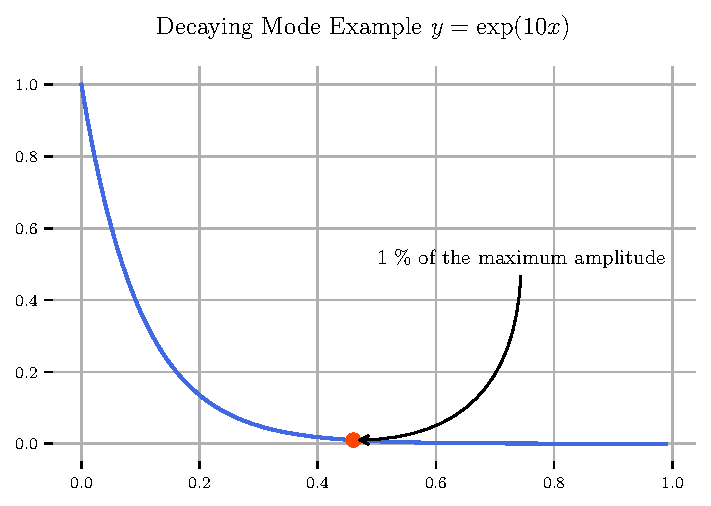
\includegraphics[width=\textwidth]{/home/jeff-severino/SWIRL/CodeRun/04-plotReport/tex-outputs/desired_cut_off_location_1_percent_of_max.pdf}
%      \caption{Decaying mode with $k_x = 0 + 10j$ and unit amplitude. One percent
%      of the maximum amplitude is identified for nacelle length comparison}
%      \label{fig:decaying_mode_with_1_percent_amp}
%  \end{figure}
 
 
% In general,
% \begin{align*}
%     y_{desired} &=  e^{-k_{x,imag} x_{desired} }\\
%     -\frac{ln|y_{desired}|}{k_{x,imag}} &=  x_{desired}
% \end{align*}
\section{Analytical Test Case}
\begin{table}[h!]
    \centering
    \begin{tabular}{|l|l|}
        \hline
        $\sigma$ & \textit{0.25} \\ \hline
        $k$      & \textit{10}   \\ \hline
        $m$      & \textit{2}    \\ \hline
        $M_x$    & \textit{0.3}  \\ \hline
    \end{tabular}
    \caption{Validation test case parameters, Uniform Flow Annular Duct} 
\end{table}

\subsection{Axial Wavenumber}
\begin{figure}
    \centering
    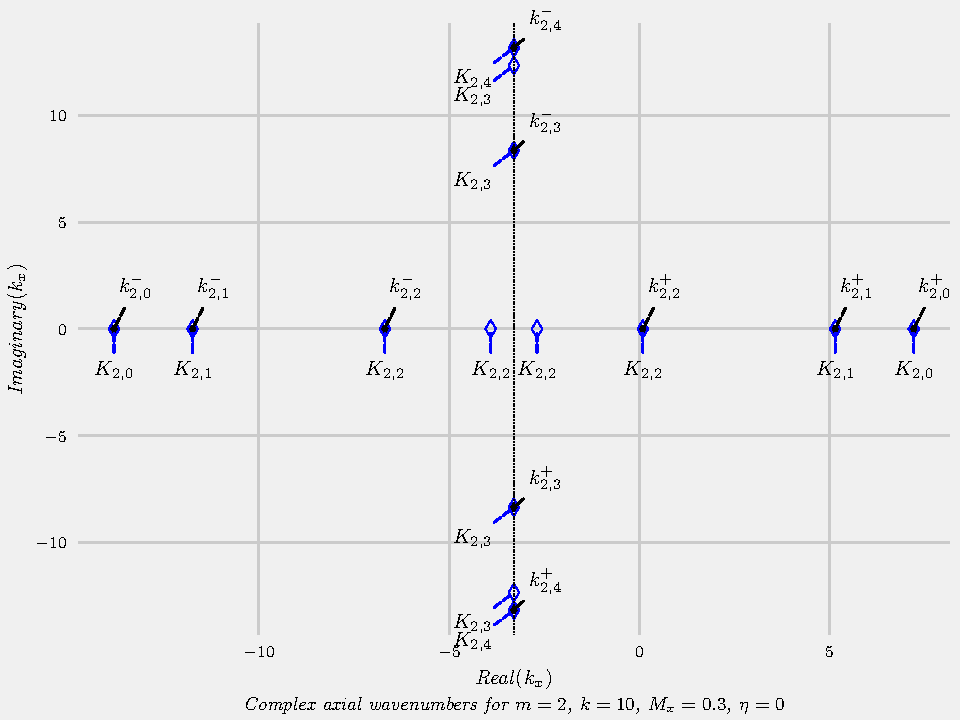
\includegraphics[width=\textwidth]{/home/jeff-severino/SWIRL/SourceFiles/PythonFiles/AnalyticalSolution_JS/figures/axial_wavenumber_analytical_test_case_comparison32gridpoints}
    \caption{Propagating Axial Wavenumbers for the analytical solution; Uniform
    Flow in a hard-wall annular duct}
    \label{fig:analytical_bessel_function}
\end{figure}


\subsection{Propagating Radial Modes}
\foreach \i in {0,...,1}
{
    \begin{figure}
        \centering
        \includegraphics[width=\textwidth]{/home/jeff-severino/SWIRL/SourceFiles/PythonFiles/AnalyticalSolution_JS/figures/radial_mode_0_test_case_number_\i.pdf}
        \caption{Propagating Axial Wavenumbers for the analytical solution; Uniform
        Flow in a hard-wall annular duct}
        \label{fig:analytical_bessel_function}
    \end{figure}
}

\foreach \i in {0,...,1}
{
    \begin{figure}
        \centering
        \includegraphics[width=\textwidth]{/home/jeff-severino/SWIRL/SourceFiles/PythonFiles/AnalyticalSolution_JS/figures/radial_mode_1_test_case_number_\i.pdf}
        \caption{Propagating Axial Wavenumbers for the analytical solution; Uniform
        Flow in a hard-wall annular duct}
        \label{fig:analytical_bessel_function}
    \end{figure}
}

\foreach \i in {0,...,3}
{
    \begin{figure}
        \centering
        \includegraphics[width=\textwidth]{/home/jeff-severino/SWIRL/SourceFiles/PythonFiles/AnalyticalSolution_JS/figures/radial_mode_2_test_case_number_\i.pdf}
        \caption{Propagating Axial Wavenumbers for the analytical solution; Uniform
        Flow in a hard-wall annular duct}
        \label{fig:analytical_bessel_function}
    \end{figure}
}

\foreach \i in {0,...,3}
{
    \begin{figure}
        \centering
        \includegraphics[width=\textwidth]{/home/jeff-severino/SWIRL/SourceFiles/PythonFiles/AnalyticalSolution_JS/figures/radial_mode_3_test_case_number_\i.pdf}
        \label{fig:analytical_bessel_function}
    \end{figure}
}

\foreach \i in {0,...,1}
{
    \begin{figure}
        \centering
        \includegraphics[width=\textwidth]{/home/jeff-severino/SWIRL/SourceFiles/PythonFiles/AnalyticalSolution_JS/figures/radial_mode_4_test_case_number_\i.pdf}
        \label{fig:analytical_bessel_function}
    \end{figure}
}

% \foreach \i in {0,...,1}
% {
%     \begin{figure}
%         \centering
%         \includegraphics[width=\textwidth]{/home/jeff-severino/SWIRL/SourceFiles/PythonFiles/AnalyticalSolution_JS/figures/radial_mode_0_test_case_number_\i.pdf}
%         \caption{Propagating Axial Wavenumbers for the analytical solution; Uniform
%         Flow in a hard-wall annular duct}
%         \label{fig:analytical_bessel_function}
%     \end{figure}
% }
% \foreach \i\j in {0,...,4}
% {
%     \begin{figure}
%         \centering
%         \includegraphics[width=\textwidth]{/home/jeff-severino/SWIRL/SourceFiles/PythonFiles/AnalyticalSolution_JS/figures/radial_mode_\i_test_case_number_1.pdf}
%         \caption{Propagating Axial Wavenumbers for the analytical solution; Uniform
%         Flow in a hard-wall annular duct}
%         \label{fig:analytical_bessel_function}
%     \end{figure}
% }
% \foreach \i\j in {2,...,3}
% {
%     \begin{figure}
%         \centering
%         \includegraphics[width=\textwidth]{/home/jeff-severino/SWIRL/SourceFiles/PythonFiles/AnalyticalSolution_JS/figures/radial_mode_\i_test_case_number_2.pdf}
%         \caption{Propagating Axial Wavenumbers for the analytical solution; Uniform
%         Flow in a hard-wall annular duct}
%         \label{fig:analytical_bessel_function}
%     \end{figure}
% }
% \foreach \i\j in {4}
% {
%     \begin{figure}
%         \centering
%         \includegraphics[width=\textwidth]{/home/jeff-severino/SWIRL/SourceFiles/PythonFiles/AnalyticalSolution_JS/figures/radial_mode_\i_test_case_number_0.pdf}
%         \caption{Propagating Axial Wavenumbers for the analytical solution; Uniform
%         Flow in a hard-wall annular duct}
%         \label{fig:analytical_bessel_function}
%     \end{figure}
% }
%  \begin{figure}
%      \centering
%      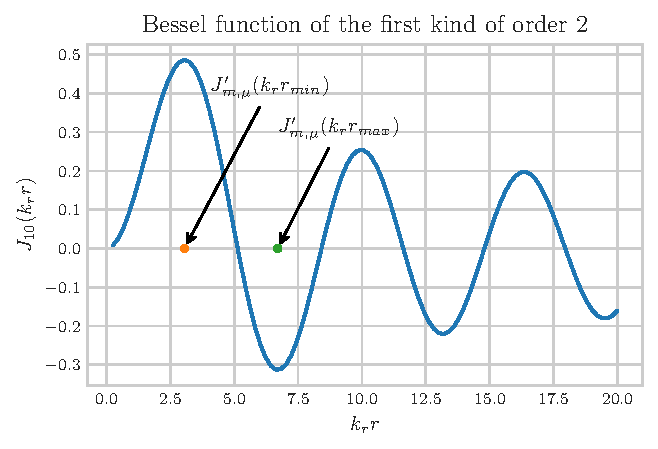
\includegraphics[width=\textwidth]{/home/jeff-severino/SWIRL/CodeRun/04-plotReport/tex-outputs/analytical_bessel_function.pdf}
%      \caption{Propagating Axial Wavenumbers for the analytical solution; Uniform
%      Flow in a hard-wall annular duct}
%      \label{fig:analytical_bessel_function}
%  \end{figure}


\end{document}


